\section{Results}
\label{sec:results}
\subsection{Survey results}
\label{sec:surveyres}
Of the \nSurvey{} respondents, \nLA{} (\shareLA\%) use lead-acid batteries, \nPW{} (\sharePW\%) reported a ``Powder'' battery of unconfirmed chemistry, and only \nLFP{} (\shareLFP\%) use LFP (\figref{survey1}, Table~\ref{tab:survey}). If Powder is a lead-based variant, lead-based batteries account for 38 of 43 drivers (88\%). The commonest set has four batteries (\fourBat{} of \nSurvey{} drivers), \onePerDay{} of \nSurvey{} charge once a day, and mean daily distance is \kmAll{} km (lead-acid \kmMeanLA{}, LFP \kmMeanLFP{}, Powder \kmMeanPW{} km; \figref{survey2}).
\begin{figure}[t]
\centering
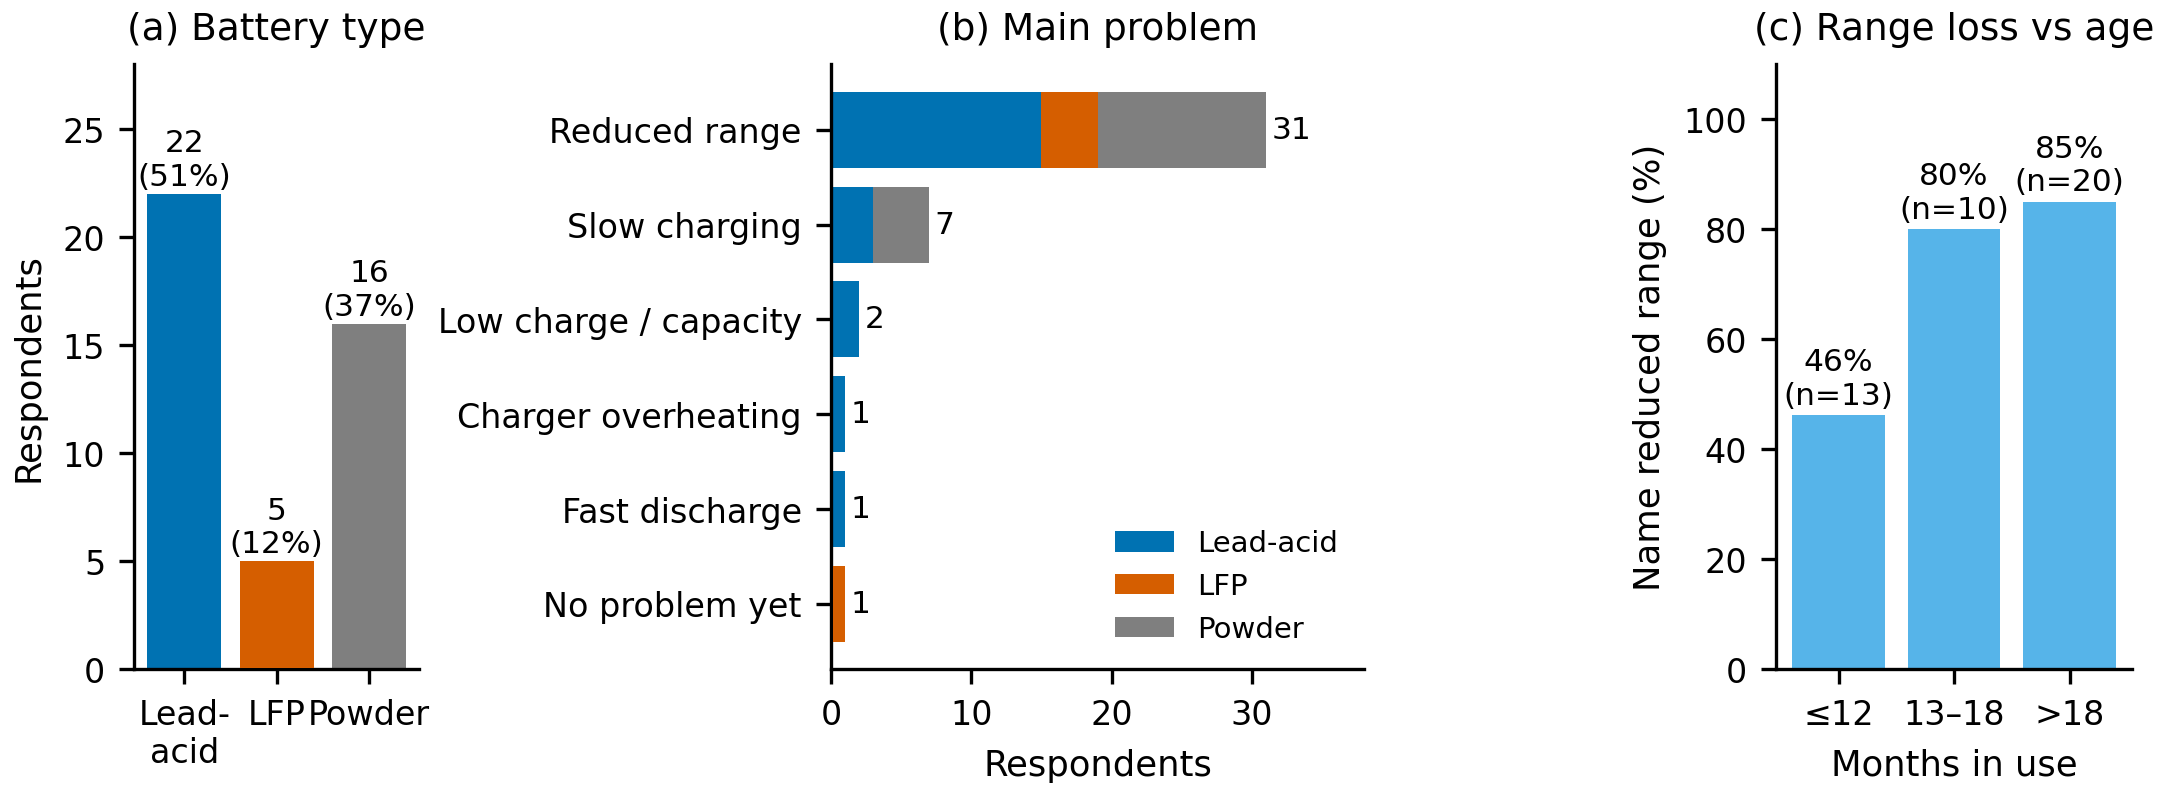
\includegraphics[width=\textwidth]{fig_survey_overview.png}
\caption{Survey sample ($n$ = 43): (a) battery type; (b) main problem reported by type; (c) share naming reduced range by months in use of the current set.}
\label{fig:survey1}
\end{figure}
\begin{table}[t]
\caption{Survey results by battery type ($n$ = 43 drivers, October 2026; source: author's field survey, cleaned data). Cost is the purchase price of the current set (BDT); replacement interval is the mid-point of the reported range (months; number of answers in brackets); resale is the mean of individual resale/purchase ratios.}
\label{tab:survey}
\centering\footnotesize
\resizebox{\textwidth}{!}{\begin{tabular}{lrrrrrrr}
\hline
Battery type & $n$ & Median cost & Mean cost & Daily km (mean) & Months in use (mean) & Median repl. interval & Resale / cost (\%) \\
\hline
Lead-acid & 22 & 29{,}000 & 46{,}318 & 83.0 & 14.1 & 18 (21) & 43 \\
Lithium (LFP) & 5 & 100{,}000 & 105{,}400 & 106.2 & 18.4 & 43.5 (4) & 13 \\
Powder & 16 & 28{,}000 & 32{,}906 & 56.9 & 21.0 & 30 (16) & 36 \\
All & 43 & 28{,}500 & 48{,}198 & 76.0 & 17.2 & 30 (41) & 37 \\
\hline
\end{tabular}}
\end{table}

The median purchase price of a lead-acid set is BDT \costMedLA{} against BDT \costMedLFP{} for LFP, a ratio of \costRatio. The lead-acid mean (BDT \costMeanLA{}) is much higher than the median because seven entries are BDT 60{,}000 or more, so medians are used. Drivers expect to replace a lead-acid set after a median \replMedLA{} months (mean \replMeanLA{}; range \replMinLA--\replMaxLA{}) and an LFP set after \replMedLFP{} months (range \replMinLFP--\replMaxLFP{}); Powder users report \replMedPW{} months. Resale value of the old set is \resaleRatioLA\% of purchase price for lead-acid and \resaleRatioLFP\% for LFP. Reduced range is the main problem for \rangeN{} of \nSurvey{} drivers (\rangeShare\%), and its share rises with the age of the set from \rngAgeA\% (up to 12 months) to \rngAgeB\% (13--18 months) and \rngAgeC\% (over 18 months; Table~\ref{tab:problems}).
\begin{figure}[t]
\centering
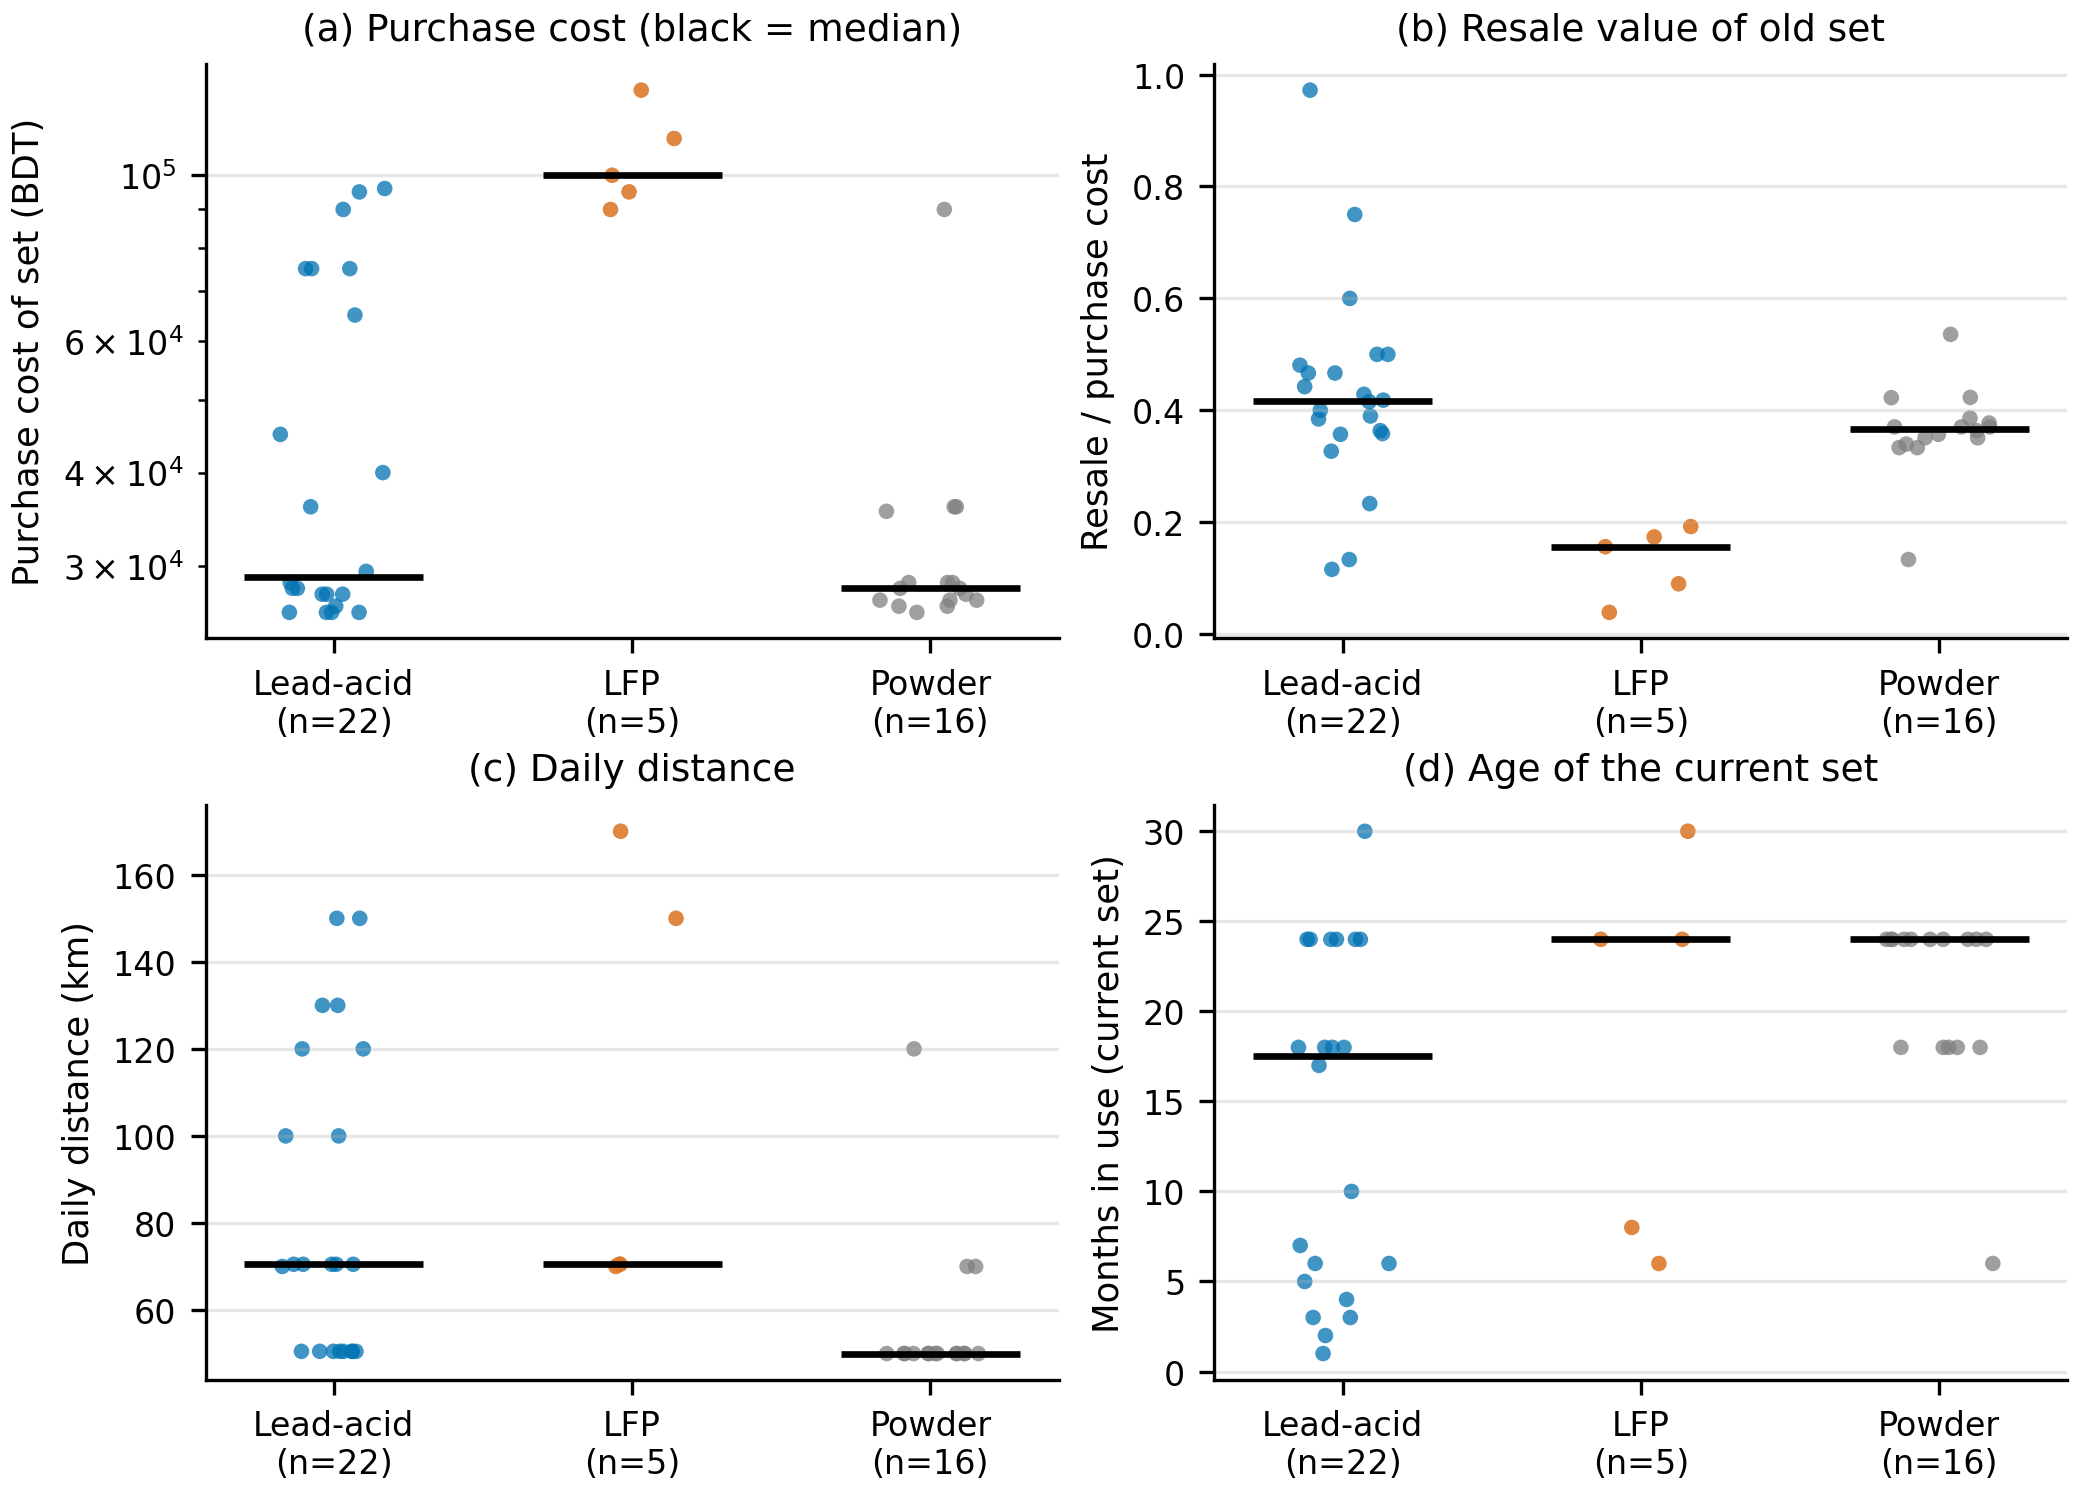
\includegraphics[width=0.9\textwidth]{fig_survey_cost_distance.png}
\caption{Survey answers by battery type (points; black bars = medians): (a) purchase cost of the current set (log scale); (b) resale/purchase ratio of the old set; (c) daily distance; (d) months in use.}
\label{fig:survey2}
\end{figure}
\begin{table}[t]
\caption{Main problem reported with the current battery (one answer per respondent) and, in the lower block, the share naming reduced range by battery-set age.}
\label{tab:problems}
\centering\footnotesize
\begin{tabular}{lrrrrr}
\hline
Problem & Lead-acid & LFP & Powder & All & Share (\%) \\
\hline
Reduced range & 15 & 4 & 12 & 31 & 72.1 \\
Slow charging & 3 & 0 & 4 & 7 & 16.3 \\
Low charge / capacity & 2 & 0 & 0 & 2 & 4.7 \\
Charger overheating & 1 & 0 & 0 & 1 & 2.3 \\
Fast discharge & 1 & 0 & 0 & 1 & 2.3 \\
No problem yet & 0 & 1 & 0 & 1 & 2.3 \\
\hline
\multicolumn{6}{l}{\emph{Reduced range by age of the current set}} \\
Up to 12 months ($n$=13) & \multicolumn{4}{r}{} & 46 \\
13--18 months ($n$=10) & \multicolumn{4}{r}{} & 80 \\
Over 18 months ($n$=20) & \multicolumn{4}{r}{} & 85 \\
\hline
\end{tabular}
\end{table}


\subsection{Calibration and validation}
\label{sec:valid}
\begin{table}[t]
\caption{Model checked against the survey and published figures (Khulna). Model (literature) uses the cycle lives of the data file (400 lead-acid, 2{,}500 LFP at 80\% DoD); model (calibrated) uses the survey-anchored values.}
\label{tab:valid}
\centering\footnotesize
\resizebox{\textwidth}{!}{\begin{tabular}{lrrrl}
\hline
Quantity & Survey / published & Model (literature) & Model (calibrated) & Outcome \\
\hline
Lead-acid replacement interval (months) & 18 (n=21; 95\% CI 17.5--30.0) & 7.8 & 18.0 & literature value 57\% below survey; calibrated \\
LFP replacement interval (months) & 43.5 (n=4; range 30--54) & 70.6 & 43.5 & literature value 62\% above survey; calibrated \\
Grid energy per bike-day, lead-acid (kWh) & 8--9 per charge (field study); 9.6 (CLEAN); 9.2 (UNCTAD) & -- & 8.4 & independent: 9--13\% below the published figures \\
Lead-acid set price (BDT) & 29{,}000 (median, n=22) & -- & 29{,}000 & input \\
LFP set price (BDT) & 100{,}000 (median, n=5) & -- & 100{,}000 & input \\
Charges per day & 1 (42 of 43 drivers) & -- & 1 & input \\
Reduced range as main problem & 72.1\% (rising with age) & -- & -- & consistent with ageing-limited life \\
\hline
\end{tabular}}
\end{table}

With the literature cycle lives (400 lead-acid, 2{,}500 LFP) the model gives a lead-acid life of \litLifeLA{} months at Khulna, \litErrLAabs\% below the survey median of \replMedLA{} months, and an LFP life of \litLifeLFP{} months, \litErrLFP\% above the survey median of \replMedLFP{} months (\figref{validlife}, Table~\ref{tab:valid}). The literature values therefore understate field life for lead-acid and overstate it for LFP. Fitting $N_{80}$ to the survey medians gives \NcalLA{} cycles for lead-acid and \NcalLFP{} for LFP. The survey interval for lead-acid has wide uncertainty (95\% bootstrap interval \ciLAlo--\ciLAhi{} months); if the ten lead-acid entries of 27 October (nine of them with the same 30-month interval) are excluded, the median is \replLAnobatch{} months ($n$ = \nLAnobatch{}). The LFP median rests on four answers (interval \ciLFPlo--\ciLFPhi{} months), and these are expectations because the sets are on average only \ageMeanLFP{} months old.
\begin{figure}[t]
\centering
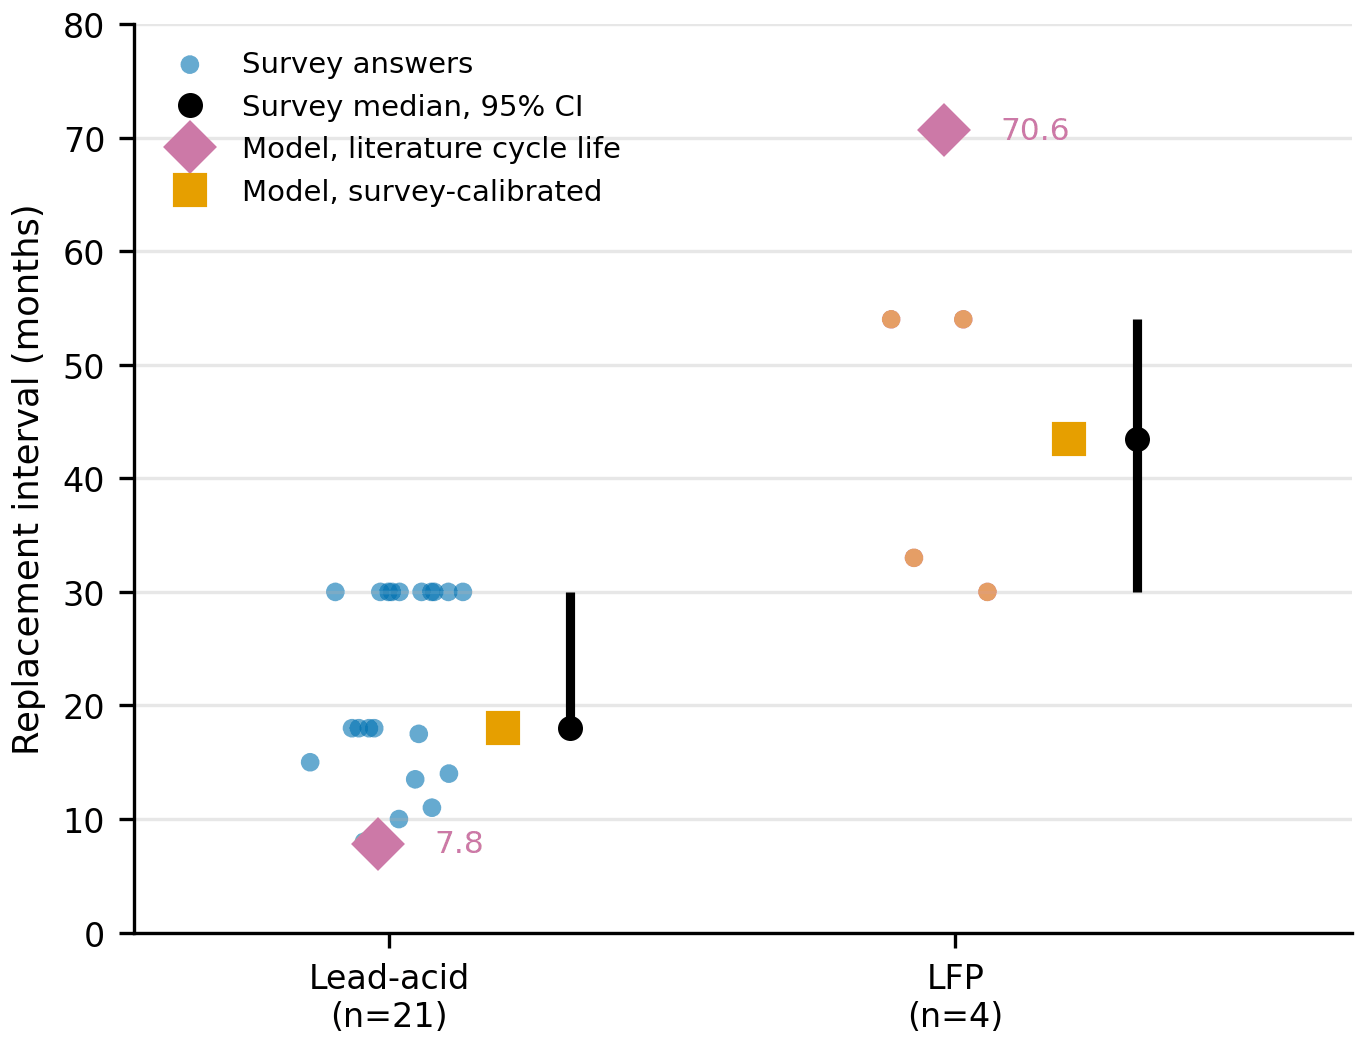
\includegraphics[width=0.6\textwidth]{fig_valid_life.png}
\caption{Validation of battery life at Khulna: survey replacement intervals (points), survey median with 95\% bootstrap interval, the model with literature cycle lives (diamond) and the survey-calibrated model (square).}
\label{fig:validlife}
\end{figure}
Three checks are independent of the calibration. Modelled lead-acid grid energy is \vEgrid{} kWh per bike-day, inside the 8--9 kWh per charge reported by the field study \cite{chowdhury2026} and \vCleanPct\% below the \vClean{} kWh implied by the CLEAN totals \cite{clean2024} and \vUnctadPct\% below the \vUnctad{} kWh per vehicle-day implied by 4{,}600 MWh/day for an estimated 500{,}000 autorickshaws, a figure reported by UNCTAD from Al-Amin and Sahabuddin \cite{unctad_smep,alamin2023} (the same brief's highlight box attributes it to 4 M vehicles, which is inconsistent and is not used). The Simulink and analytic models agreed in all twelve cases of the verification run (Appendix~\ref{app:sim}). Finally, the rise in range complaints with age (\figref{survey1}c) is consistent with ageing-limited life. The model is therefore checked against survey and published ranges, but it is not validated against metered operating data.

\subsection{Temperature and battery performance}
Monthly mean T2M follows the same seasonal cycle at all three sites, from about \Tmin\,$^\circ$C in January to \Tmax\,$^\circ$C in April 2024 (\figref{temp}). Mean battery temperature is \TcKhulna, \TcChuadanga\ and \TcRajshahi\,$^\circ$C, a spread of \Tspread\,$^\circ$C. Because the calibration is made at Khulna, modelled life differs between sites only through temperature: \lifeLAKhulna, \lifeLAChuadanga\ and \lifeLARajshahi{} months for lead-acid and \lifeLFPKhulna, \lifeLFPChuadanga\ and \lifeLFPRajshahi{} months for LFP (Table~\ref{tab:results}).
\begin{figure}[t]
\centering
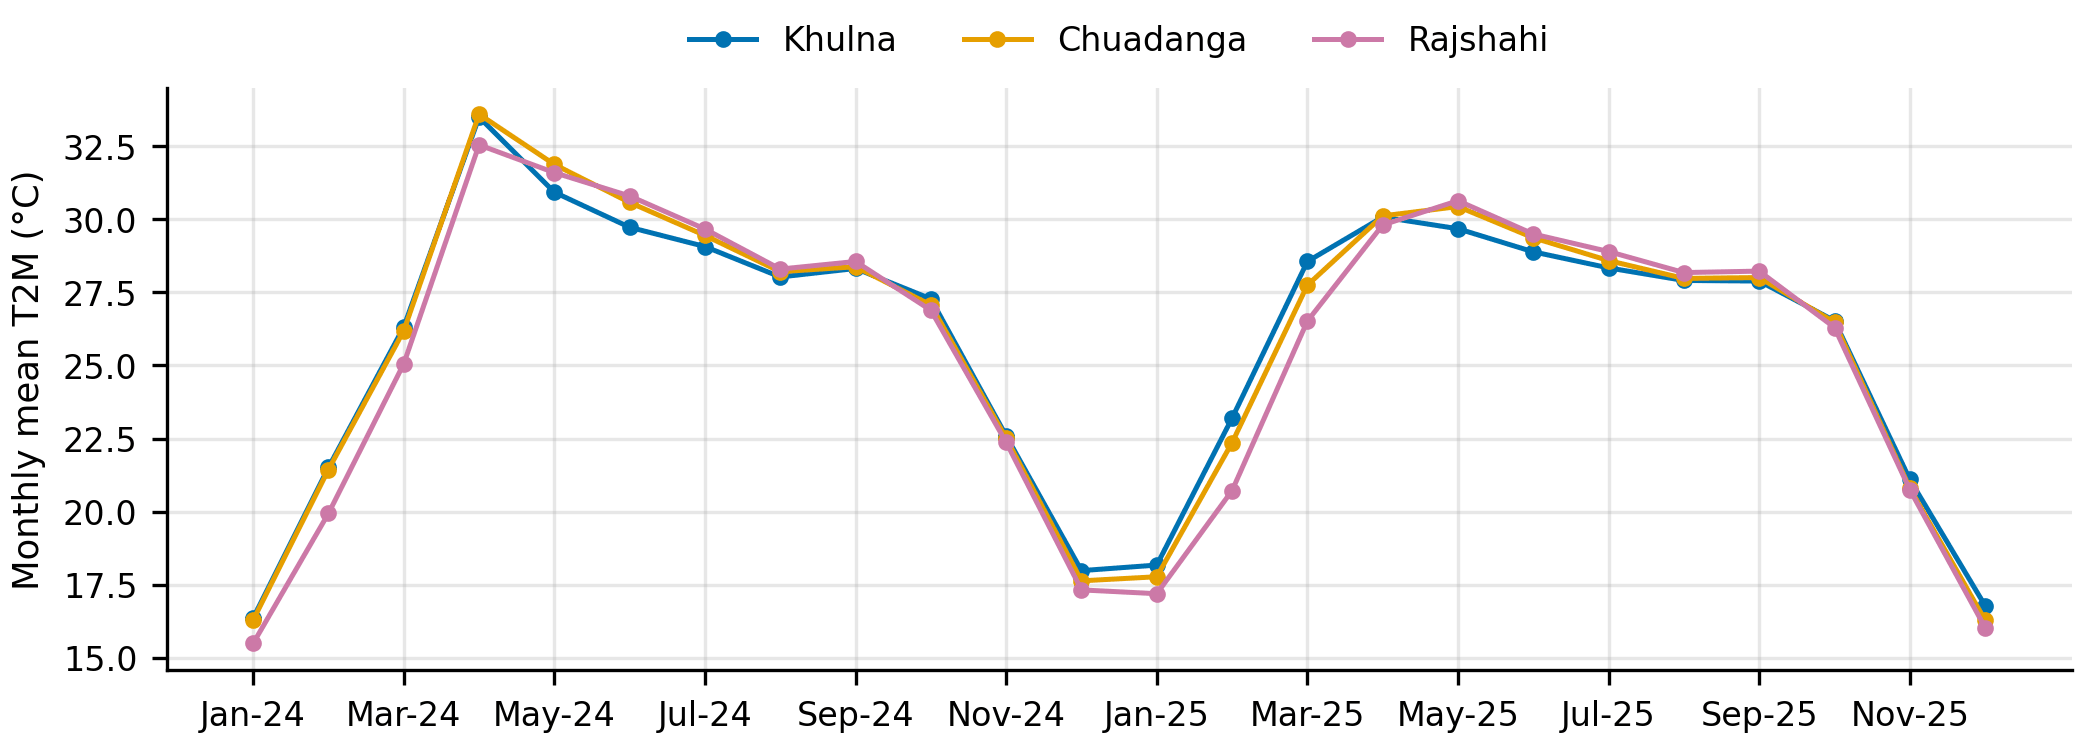
\includegraphics[width=0.9\textwidth]{fig1_temperature.png}
\caption{NASA POWER monthly mean 2\,m temperature at the three sites, Jan 2024--Dec 2025.}
\label{fig:temp}
\end{figure}
\begin{table}[t]
\caption{Survey-anchored model results for three sites (NASA POWER monthly $T_{2m}$, Jan 2024--Dec 2025; battery temperature = ambient + 5\,$^\circ$C). Cycle life is calibrated at Khulna so that modelled life equals the survey median replacement interval (18 months lead-acid, 43.5 months LFP); other sites differ only through temperature. TCO is net present cost at 11.96\% discount rate and BDT 11.36/kWh. Source: \texttt{results\_summary.csv} from \texttt{easybike\_main.m}.}
\label{tab:results}
\centering\footnotesize
\resizebox{\textwidth}{!}{\begin{tabular}{llrrrrrrrrr}
\hline
Site & Battery & $\bar T_{cell}$ & $\eta$ & DoD & Range & $E_{grid}$ & Life & Repl. & TCO$_{10}$ & Cost \\
 & & ($^\circ$C) & (\%) & (\%) & (km) & (kWh/d) & (mo) & (10 yr) & ($10^3$ BDT) & (BDT/km) \\
\hline
Khulna & Lead-Acid & 30.8 & 90.2 & 88.1 & 69.1 & 8.35 & 18.0 & 6 & 245 & 1.90 \\
 & LFP & 30.8 & 97.8 & 82.1 & 74.1 & 7.09 & 43.5 & 2 & 322 & 2.50 \\
\hline
Chuadanga & Lead-Acid & 30.8 & 90.2 & 88.1 & 69.1 & 8.36 & 17.8 & 6 & 247 & 1.91 \\
 & LFP & 30.8 & 97.8 & 82.1 & 74.0 & 7.09 & 43.3 & 2 & 323 & 2.50 \\
\hline
Rajshahi & Lead-Acid & 30.5 & 90.0 & 88.4 & 68.9 & 8.38 & 18.1 & 6 & 246 & 1.90 \\
 & LFP & 30.5 & 97.8 & 82.2 & 74.0 & 7.09 & 43.7 & 2 & 322 & 2.49 \\
\hline
\end{tabular}}
\end{table}

Discharge efficiency is \effLA\% for lead-acid and \effLFP\% for LFP, so LFP draws \gridratio\% less grid energy (\egLA{} versus \egLFP{} kWh per day). At \kmUsed{} km per day the lead-acid set runs at \dodLA\% mean depth of discharge (maximum \dodmaxLA\%), above the 80\% limit on which cycle life is rated, which is consistent with its short life; the LFP set runs at \dodLFP\% (maximum \dodmaxLFP\%). The modelled range to 80\% DoD is \rngLA{} km for lead-acid and \rngLFP{} km for LFP.
\begin{figure}[t]
\centering
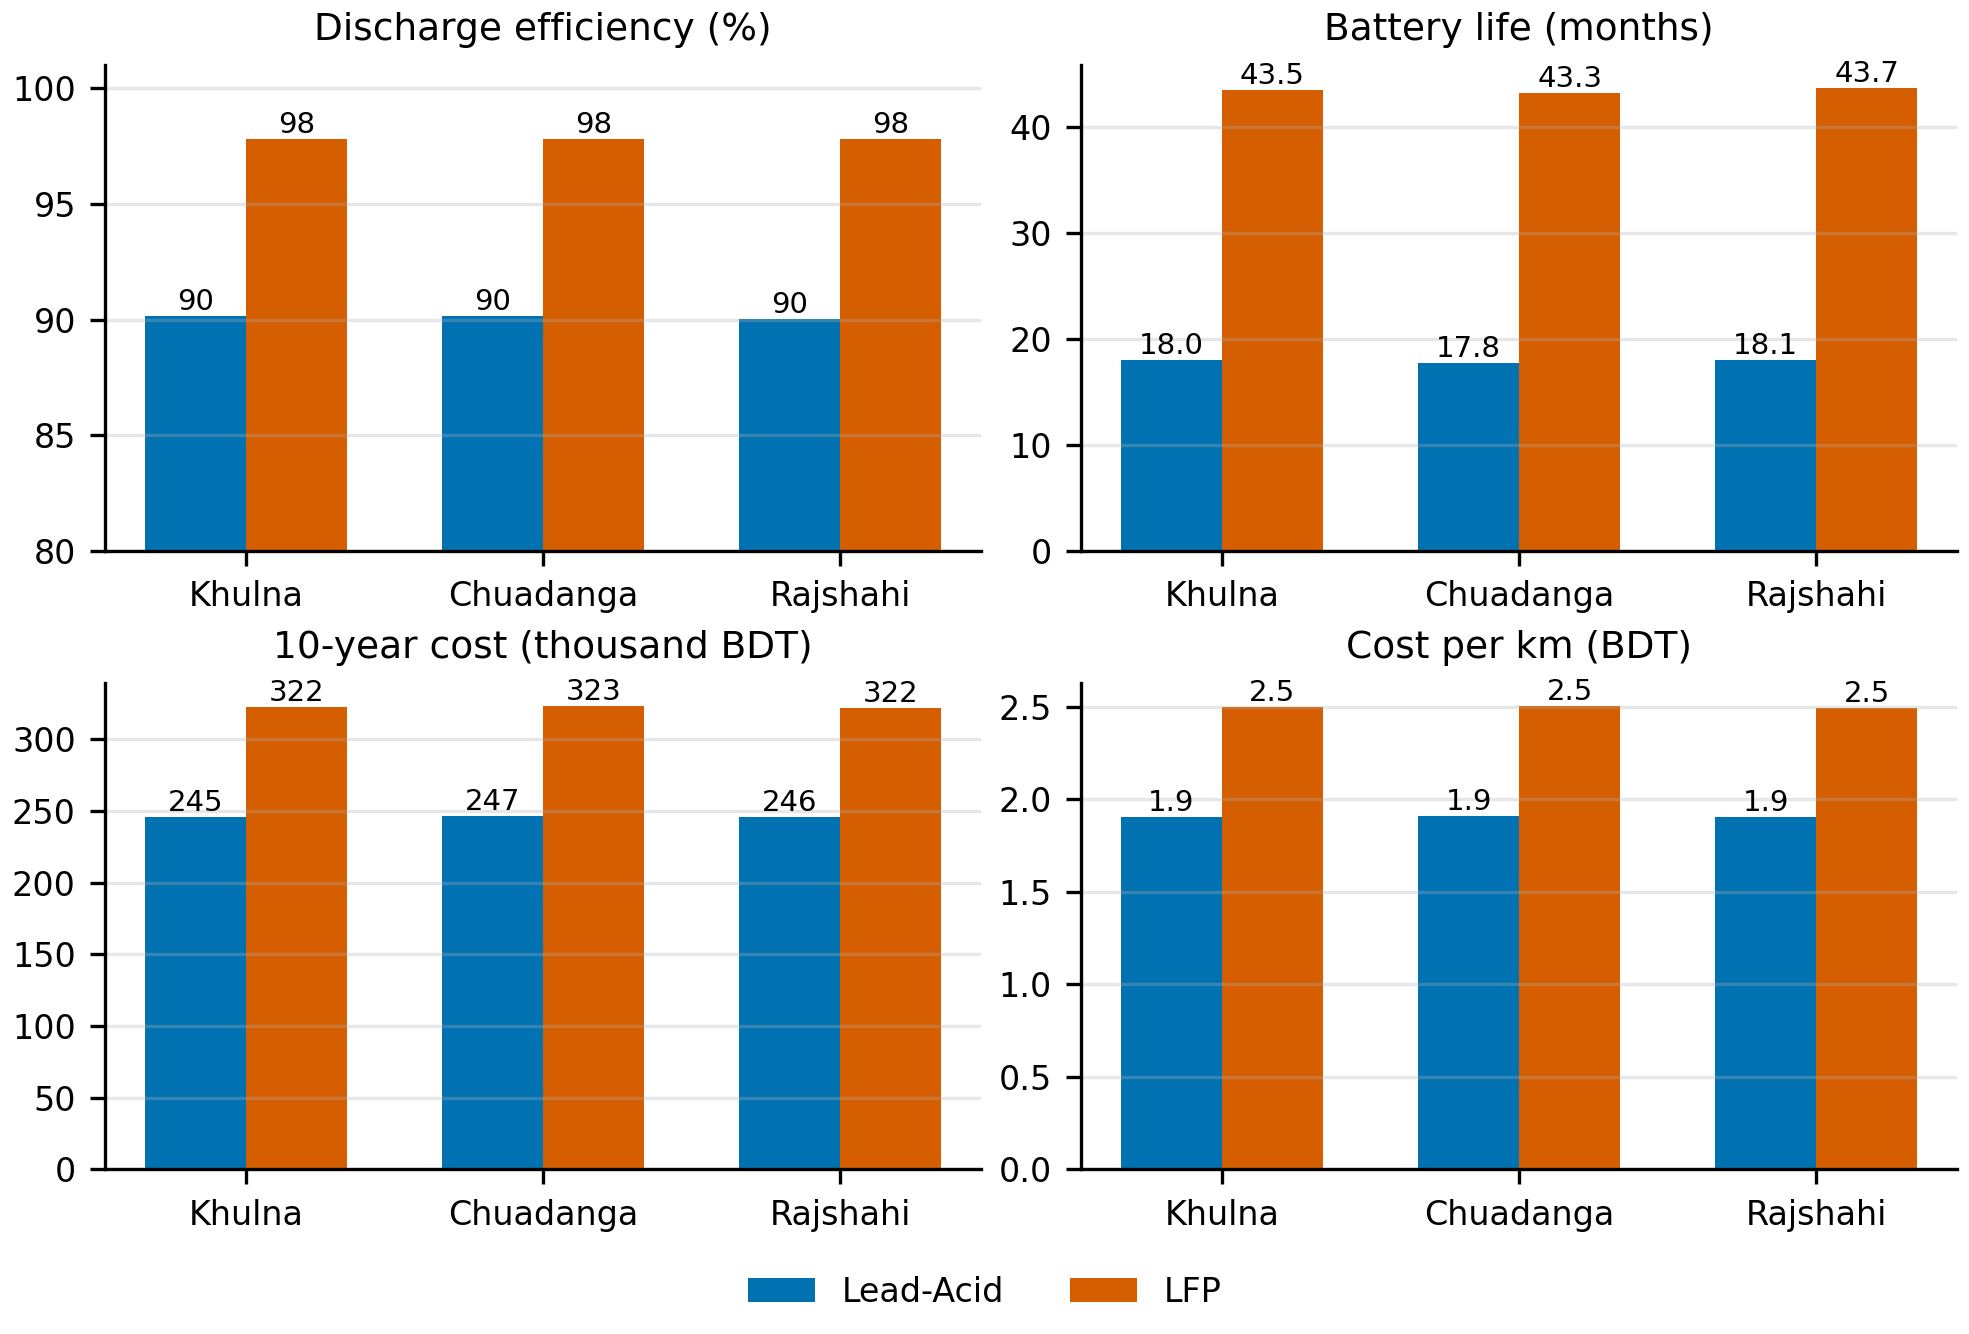
\includegraphics[width=0.85\textwidth]{fig2_comparison.png}
\caption{Site comparison of discharge efficiency, battery life, 10-year NPV cost and cost per km.}
\label{fig:comp}
\end{figure}
\begin{figure}[t]
\centering
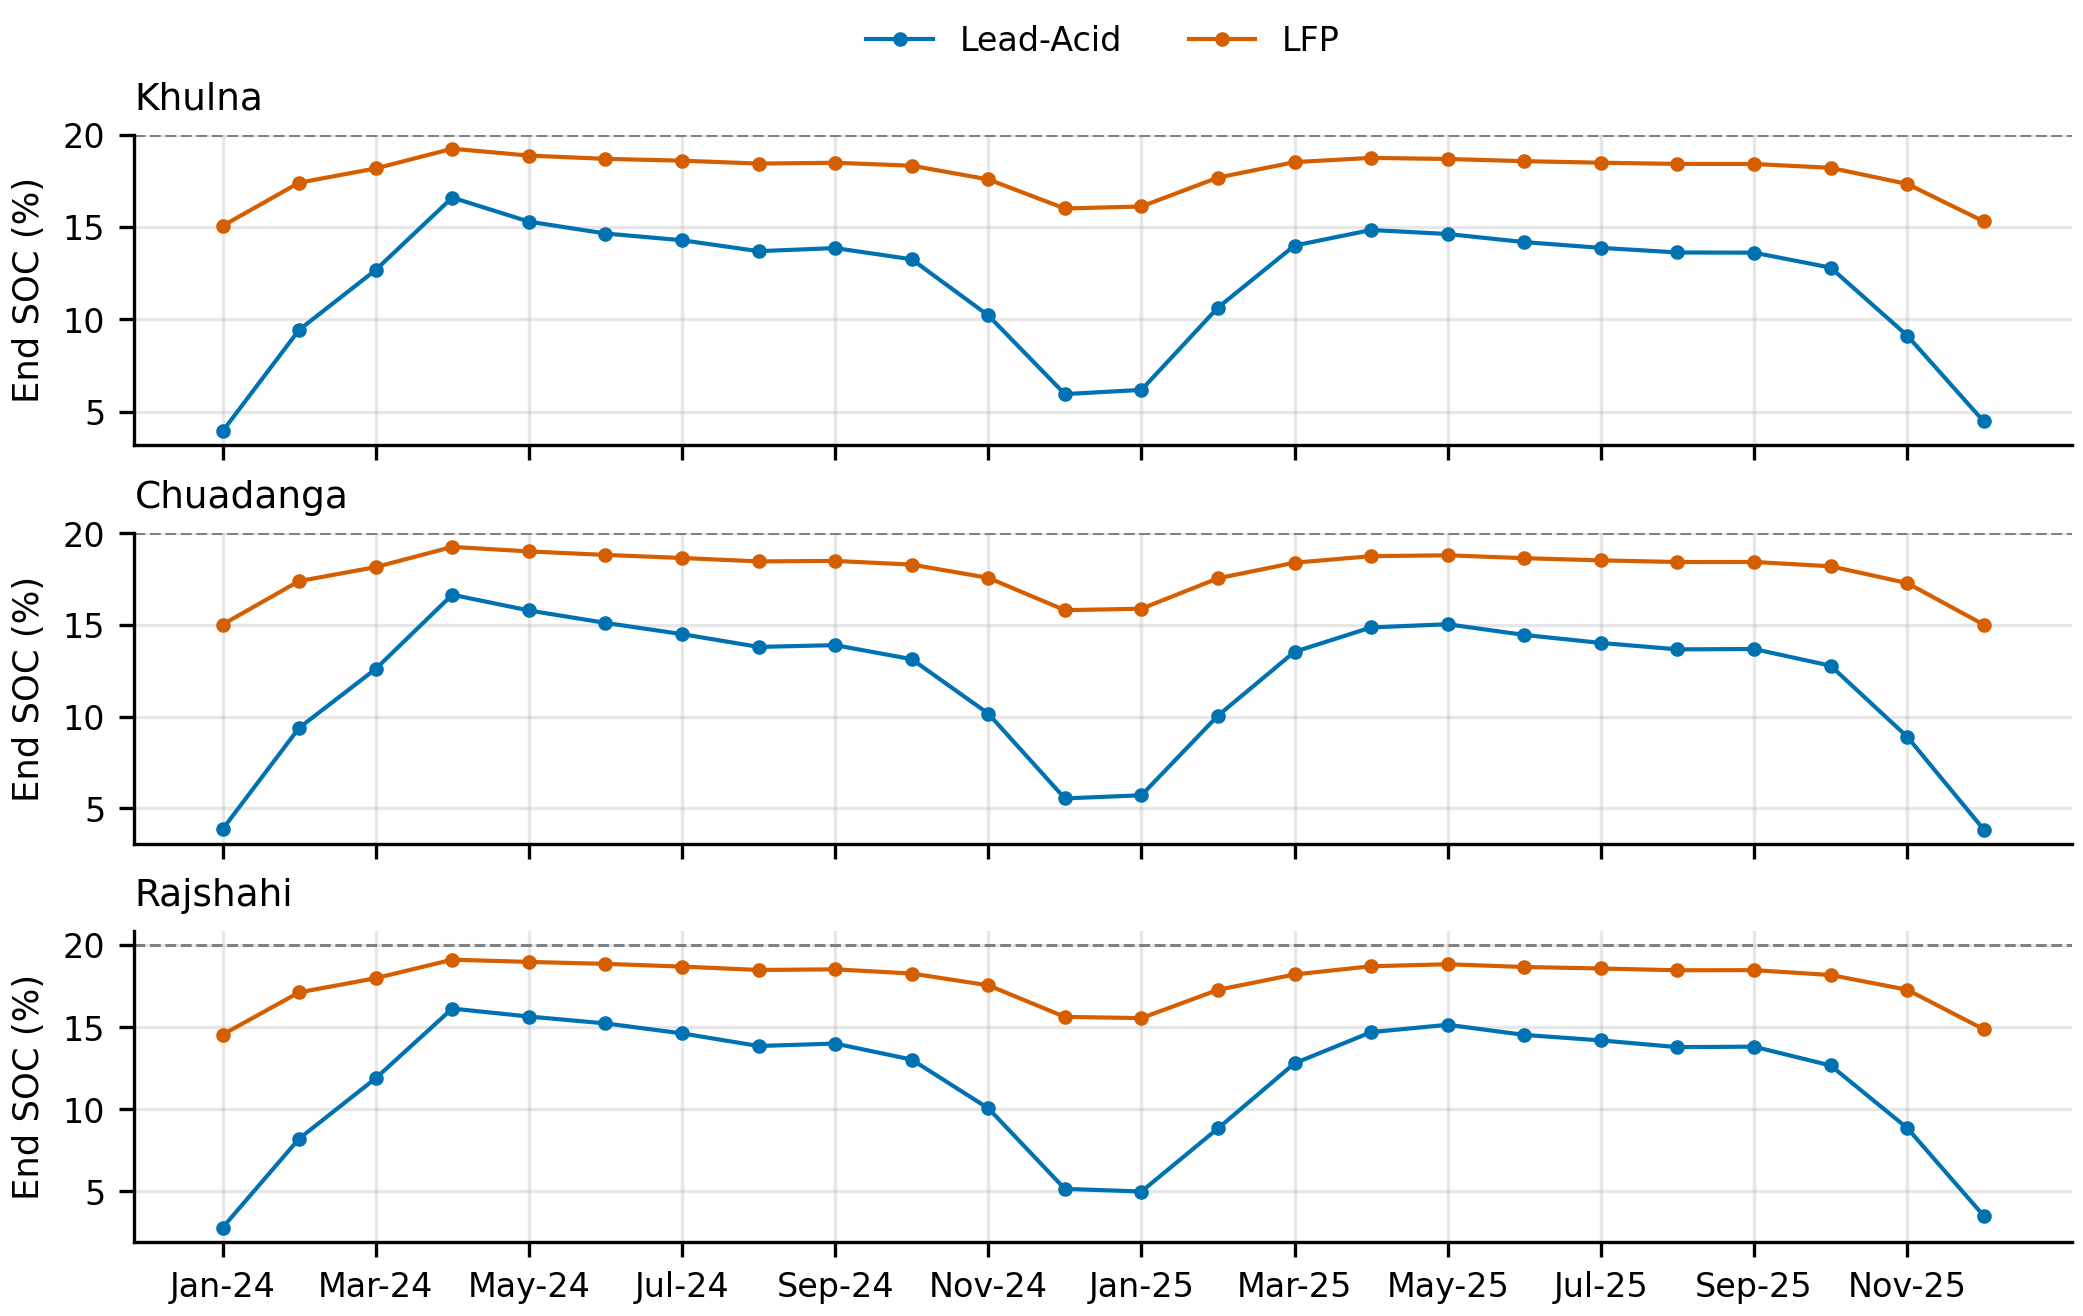
\includegraphics[width=0.85\textwidth]{fig3_soc.png}
\caption{Month-end state of charge after one day's discharge; dashed line = 20\% limit.}
\label{fig:soc}
\end{figure}

\subsection{Cost of ownership}
With survey-anchored inputs the ten-year net present cost per bike is BDT \tcoLA{} for lead-acid and BDT \tcoLFP{} for LFP (site mean): LFP costs BDT \gapLFP{} (\gapPct\%) \emph{more}, and its cost per km is BDT \cpkLFP{} against BDT \cpkLA{}. A lead-acid bike needs \repLA{} replacement sets in ten years and an LFP bike \repLFP{}, but each LFP set costs \costRatio{} times as much and is resold for a smaller share of its price (\figref{tco}). With the literature cycle lives the sign reverses: LFP would be BDT \litGap{} cheaper. Using drivers' own prices and intervals therefore changes the operator's conclusion.
\begin{figure}[t]
\centering
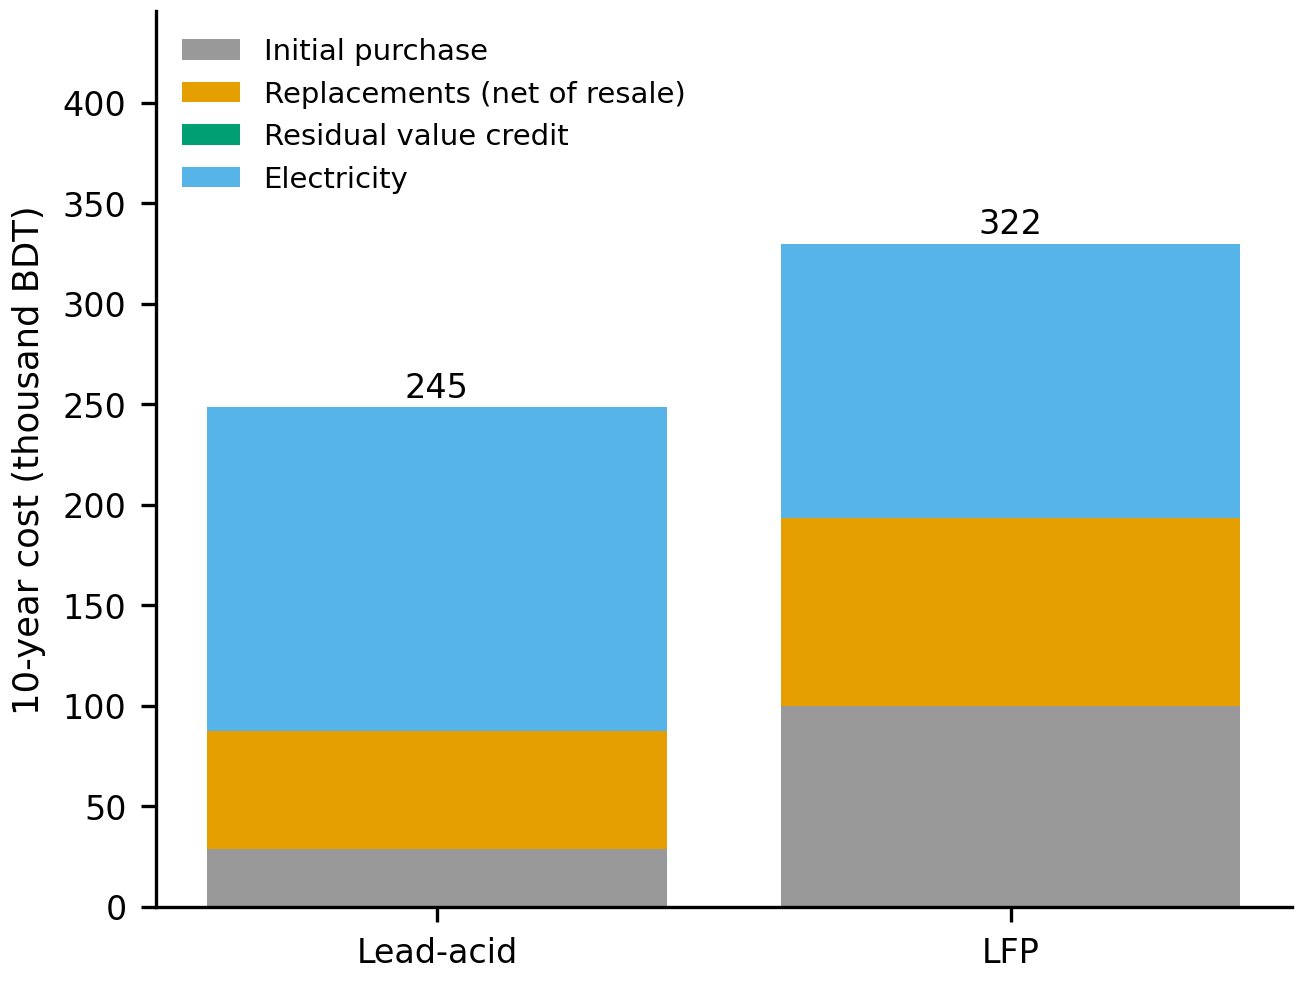
\includegraphics[width=0.55\textwidth]{fig_tco_breakdown.png}
\caption{Composition of the 10-year cost at Khulna (thousand BDT).}
\label{fig:tco}
\end{figure}

\subsection{Break-even, scenarios and sensitivity}
\label{sec:sens}
LFP matches lead-acid at a set price of BDT \beP{} (\bePpct\% below the survey median) if its life is \replMedLFP{} months, or at a life of \beL{} months if the price is BDT \priceLFP{} (\figref{breakeven}). The break-even price is BDT \bePA{} for a 30-month life, \bePB{} for 54 months, \bePC{} for 72 months and \bePD{} for 96 months. All five surveyed LFP set prices lie above the break-even line.
\begin{figure}[t]
\centering
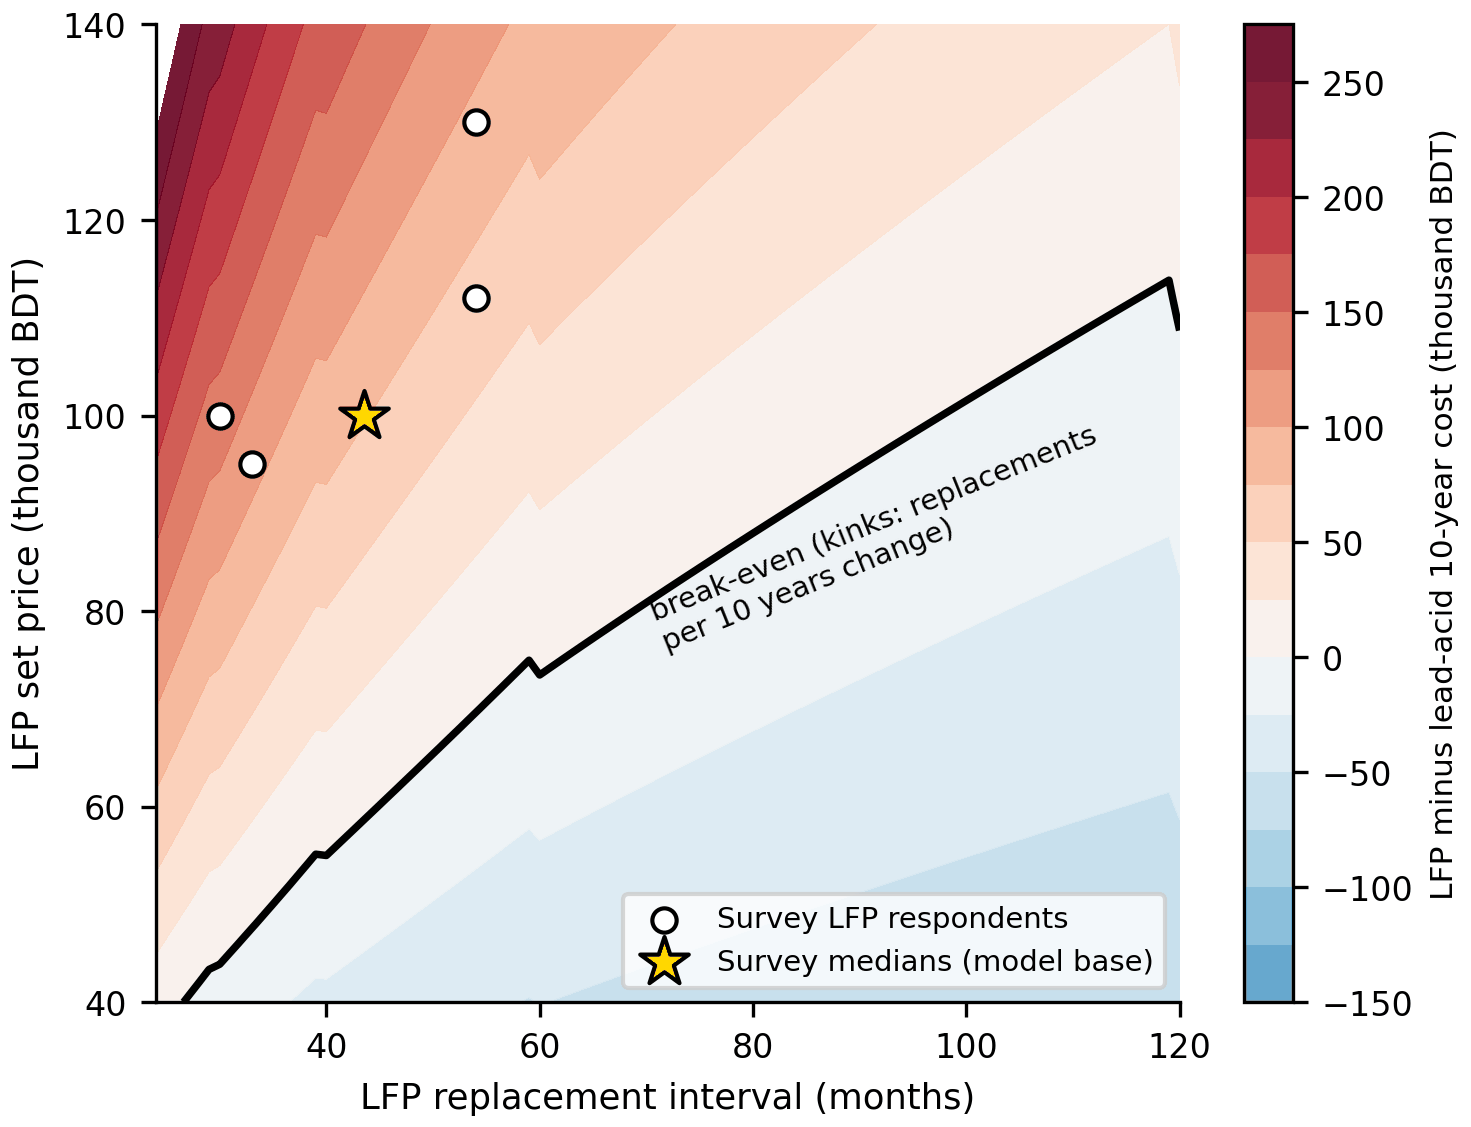
\includegraphics[width=0.62\textwidth]{fig_breakeven.png}
\caption{Ten-year cost of LFP minus lead-acid at Khulna as a function of LFP set price and replacement interval. Red: LFP dearer; blue: LFP cheaper. White circles: surveyed LFP drivers; star: survey medians. Kinks occur where the number of replacements in ten years changes.}
\label{fig:breakeven}
\end{figure}
\begin{table}[t]
\caption{Scenario runs. Upper block: battery temperature rise above ambient (site mean). Lower block: daily distance at Khulna (max DoD $>$100\% means the pack cannot serve the duty). Life in months; TCO in $10^3$ BDT.}
\label{tab:scen}
\centering\footnotesize
\resizebox{\textwidth}{!}{\begin{tabular}{lrrrrrr}
\hline
 & \multicolumn{2}{c}{Life (months)} & \multicolumn{2}{c}{10-yr TCO ($10^3$ BDT)} & \multicolumn{2}{c}{Max DoD (\%)} \\
Scenario & LA & LFP & LA & LFP & LA & LFP \\
\hline
$\Delta T$ = +0\,$^\circ$C & 23.8 & 51.6 & 236 & 300 & -- & -- \\
$\Delta T$ = +5\,$^\circ$C & 18.0 & 43.5 & 246 & 322 & -- & -- \\
$\Delta T$ = +10\,$^\circ$C & 12.5 & 35.3 & 269 & 352 & -- & -- \\
\hline
50 km/day & 32.3 & 66.1 & 161 & 229 & 63 & 56 \\
76 km/day & 18.0 & 43.5 & 245 & 322 & 96 & 85 \\
100 km/day & 12.3 & 33.1 & 328 & 408 & 126 & 112 \\
\hline
\end{tabular}}
\end{table}

Table~\ref{tab:scen} shows that battery temperature rise and daily distance change life and cost for both chemistries without changing the ranking. The tornado chart (\figref{tornado}) shows that the lead-acid life and LFP life and price dominate, and that the tariff, discount rate and operating days matter little. If lead-acid sets lasted only 8 months (the shortest survey answer) LFP would roughly break even (gap BDT \laEightGap{}); if they lasted 30 months (the longest) LFP would be BDT \laThirtyGap{} dearer. Combining the most favourable survey values for LFP (lead-acid life 8 months and price BDT 45{,}000, LFP life 54 months and price BDT 90{,}000) makes LFP BDT 147{,}457 cheaper; the most unfavourable combination makes it BDT \extUnfav{} dearer. Tariffs of BDT 7.70 and 16.24 per kWh leave the gap at BDT \tarLow{} and \tarHigh{}. A hot day at 42\,$^\circ$C ambient ages lead-acid \heatLA{} times and LFP \heatLFP{} times faster than the 2024--25 monthly-mean climate.
\begin{figure}[t]
\centering
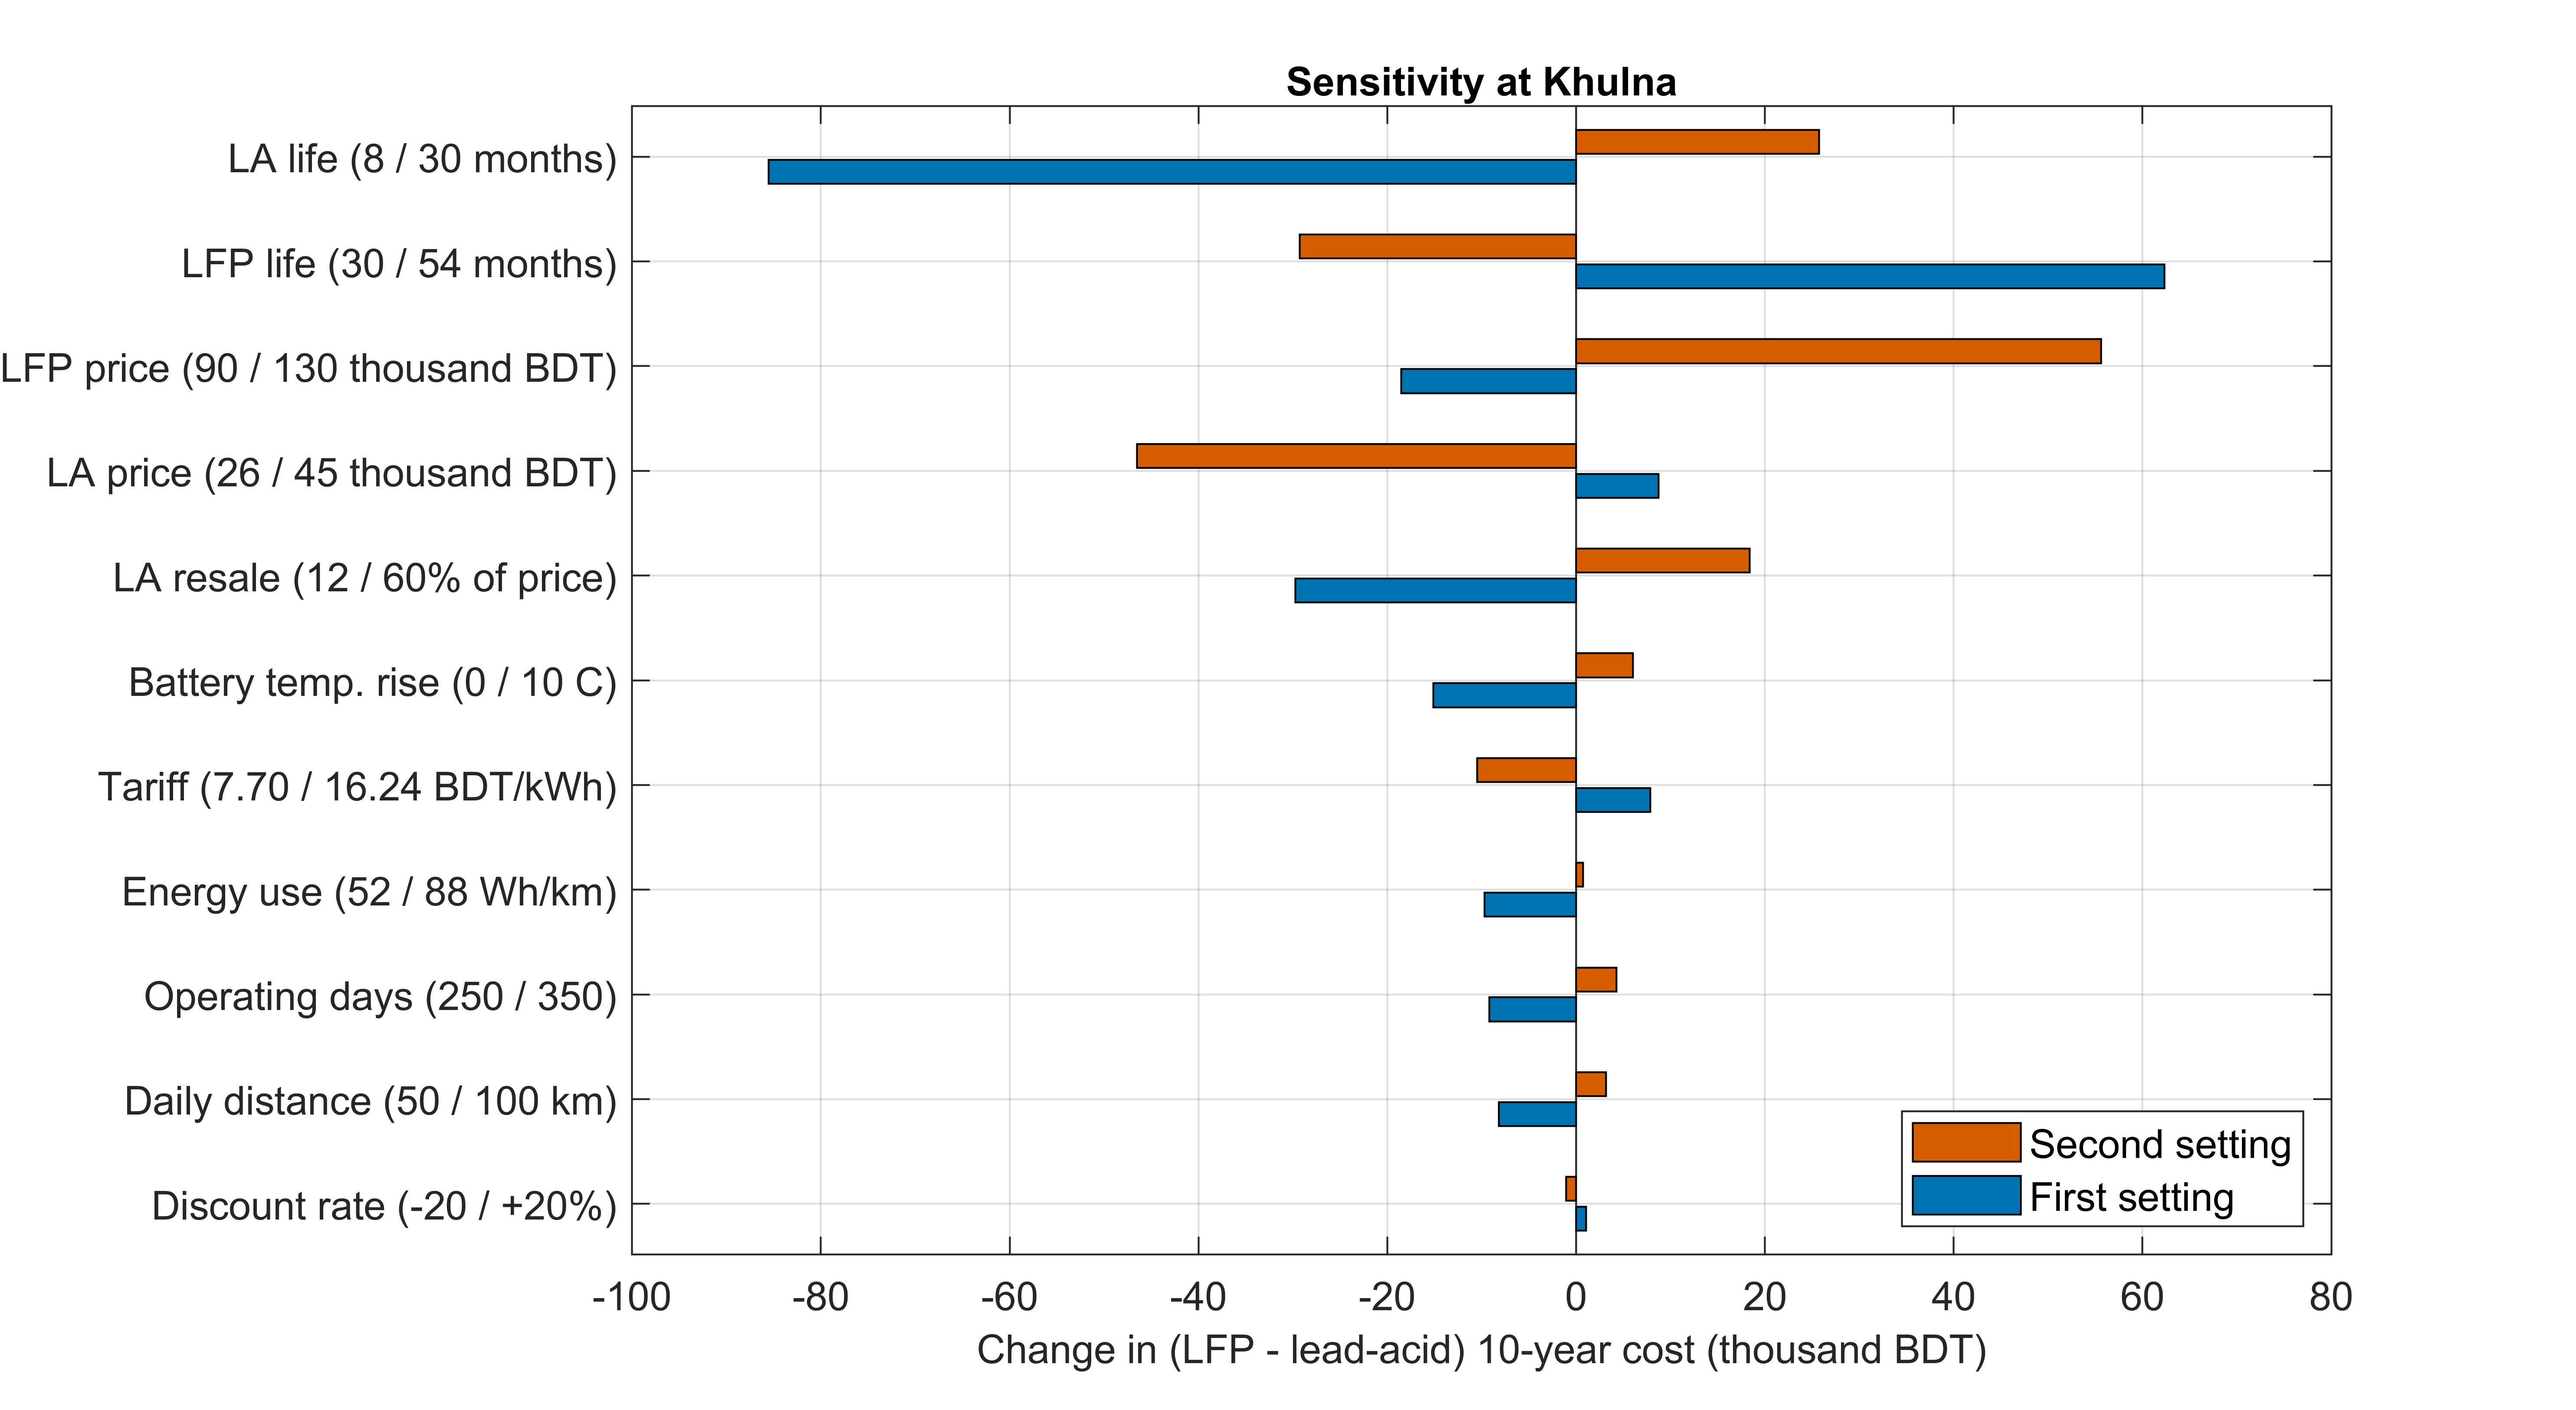
\includegraphics[width=0.9\textwidth]{fig4_tornado.png}
\caption{One-at-a-time sensitivity of the LFP-minus-LA 10-year cost gap at Khulna (base gap +\gapLFP{} BDT). Negative values favour LFP.}
\label{fig:tornado}
\end{figure}

\subsection{Carbon footprint, lead flow and policy scenarios}
A lead-acid easy-bike causes about \perbikeLA{} kg CO$_2$e per year and an LFP bike \perbikeLFP{} (Table~\ref{tab:co2bike}, \figref{co2}). Switching one bike saves \saveBike{} kg CO$_2$e per year, \saveOp{} from lower electricity use and \saveEmb{} from fewer manufactured sets (\packsLA{} lead-acid against \packsLFP{} LFP sets per year). For 1.4 M bikes this is \fleetA{} Mt CO$_2$e per year, or \fleetB{} Mt for 3 M bikes. The per-bike saving stays between \sensMin{} and \sensMax{} kg per year for LFP manufacturing footprints of 50--110 kg CO$_2$e/kWh and grid factors of 0.55--0.70 (\figref{co2sens}).
\begin{table}[t]
\caption{Carbon budget per bike per year (Khulna, survey-anchored lives; grid factor 0.62 tCO$_2$/MWh; manufacture and end-of-life 40 and 50 kg CO$_2$e per kWh of pack capacity for LA and LFP; pack energy 6.7 kWh for both).}
\label{tab:co2bike}
\centering\footnotesize
\begin{tabular}{lrrrr}
\hline
Battery & Packs/yr & Operation & Manuf.+EOL & Total \\
 & & (kg CO$_2$e) & (kg CO$_2$e) & (kg CO$_2$e) \\
\hline
Lead-acid & 0.67 & 1556 & 180 & 1736 \\
LFP & 0.28 & 1319 & 93 & 1412 \\
\hline
\end{tabular}
\end{table}

\begin{figure}[t]
\centering
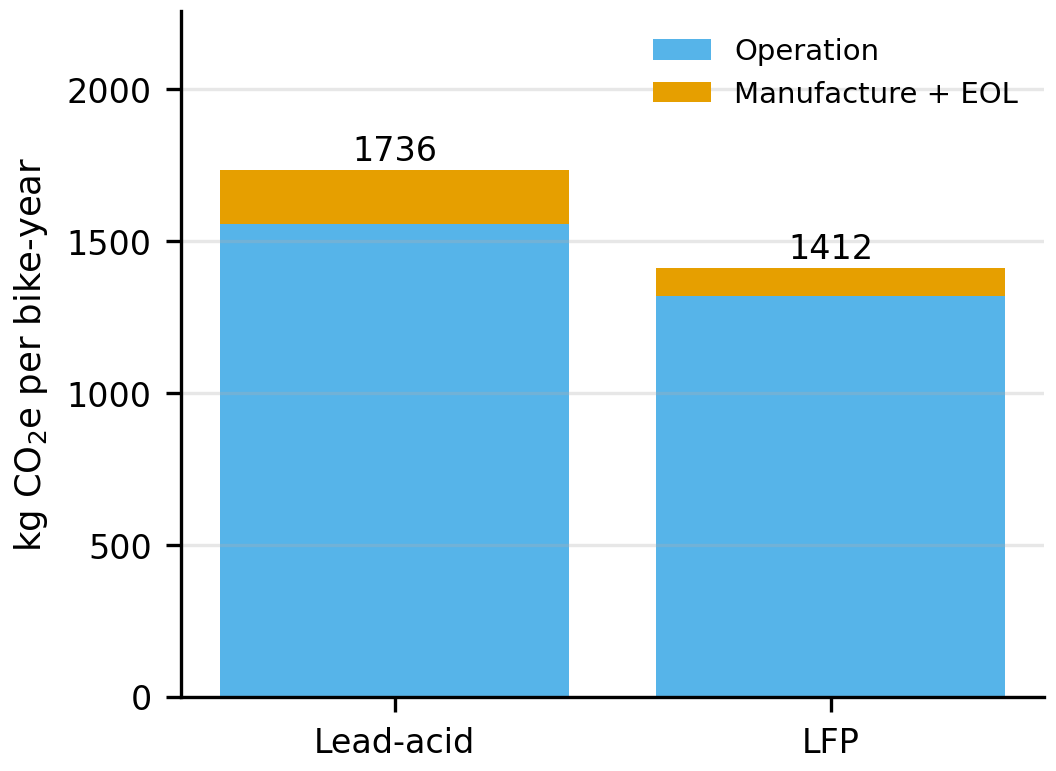
\includegraphics[width=0.45\textwidth]{fig5_co2_bike.png}\hfill
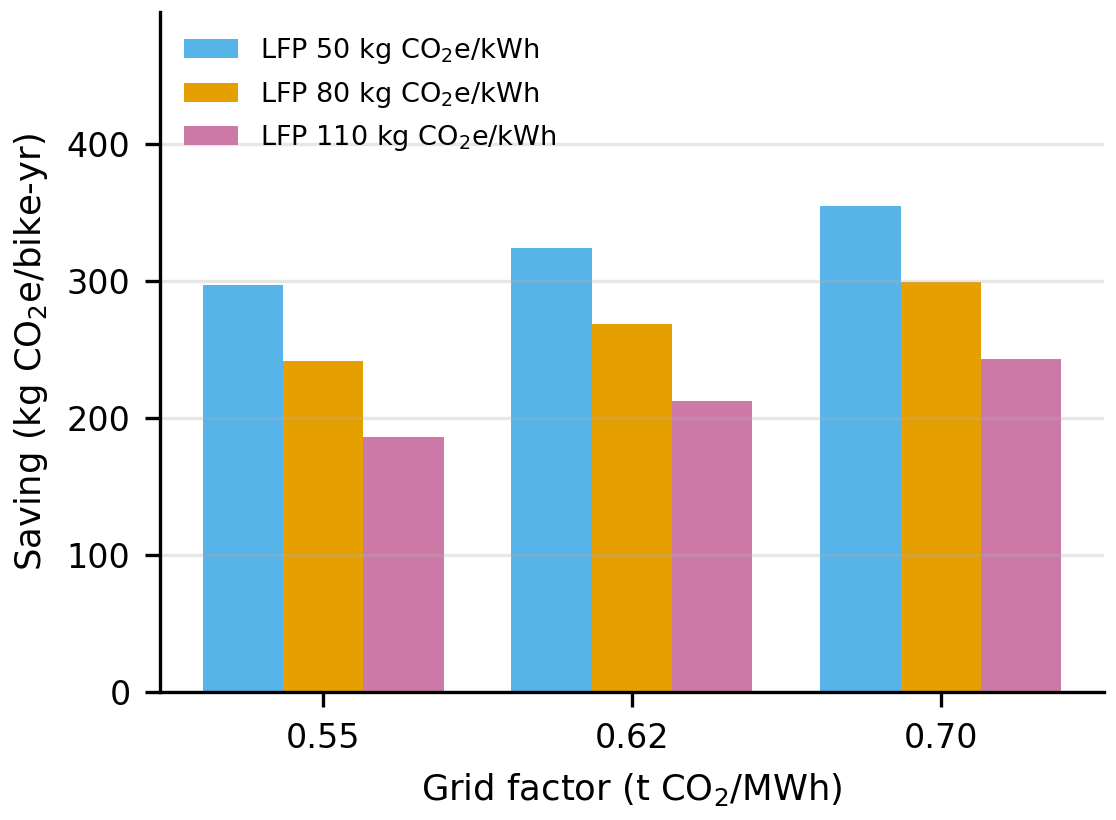
\includegraphics[width=0.45\textwidth]{fig7_co2_sensitivity.png}
\caption{Left: annual carbon footprint per bike. Right: per-bike saving from LFP for three LFP manufacturing footprints and three grid emission factors (\figref{co2sens}).}
\label{fig:co2}\label{fig:co2sens}
\end{figure}
The lead-acid fleet cycles \leadLow--\leadHigh{} kt of lead per year at 1.4 M bikes (Table~\ref{tab:lead}), or \leadBikeLow--\leadBikeHigh{} kg per bike-year; the upper value is close to the 167 kt reported by Pure Earth for recycling in the whole sector \cite{pureearth_smep}. Converted bikes need replacement so rarely that their lead flow in the model is negligible. Because LFP is dearer for the operator, conversion needs support: BDT \suppHalf{} billion over ten years for 50\% conversion and BDT \suppFull{} billion for full conversion (Table~\ref{tab:policy}, \figref{policy}). Per tonne of CO$_2$e saved the implied cost is BDT \abateCarbon{}, and per kilogram of lead kept out of recycling BDT \abateLead{} (BDT \abateLeadLow--\abateLeadHigh{} for 125 and 56 kg per set). These figures count only operator cost; they exclude the health benefits of less lead.
\begin{table}[t]
\caption{Lead throughput of the lead-acid fleet (kt Pb per year through replacement and recycling) at the survey replacement interval. 56 and 84 kg correspond to a four-battery set at 14 and 21 kg lead per battery; 125 kg is the Pure Earth figure.}
\label{tab:lead}
\centering\footnotesize
\begin{tabular}{lrr}
\hline
Lead per set & 1.4 M bikes & 3.0 M bikes \\
\hline
56 kg & 52 & 112 \\
84 kg & 79 & 168 \\
125 kg & 117 & 251 \\
\hline
\end{tabular}
\end{table}

\begin{table}[t]
\caption{Conversion scenarios for a 1.4 M-bike fleet (share moved from lead-acid to LFP). Lead flow assumes 84 kg Pb per lead-acid set (56--125 kg, Table~\ref{tab:lead}). Operator support is the 10-year cost difference that must be covered for LFP to match lead-acid.}
\label{tab:policy}
\centering\footnotesize
\setlength{\tabcolsep}{3pt}
\begin{tabular}{lrrrr}
\hline
Scenario & Share & CO$_2$e saved & Pb cycled & Support needed \\
 & (\%) & (Mt/yr) & (kt/yr) & ($10^9$ BDT) \\
\hline
S0 Business as usual & 0 & 0.00 & 79 & 0 \\
S1 Early adoption & 25 & 0.11 & 59 & 27 \\
S2 Targeted policy & 50 & 0.23 & 39 & 53 \\
S3 Full transition & 100 & 0.45 & 0 & 107 \\
\hline
\end{tabular}
\end{table}

\begin{figure}[t]
\centering
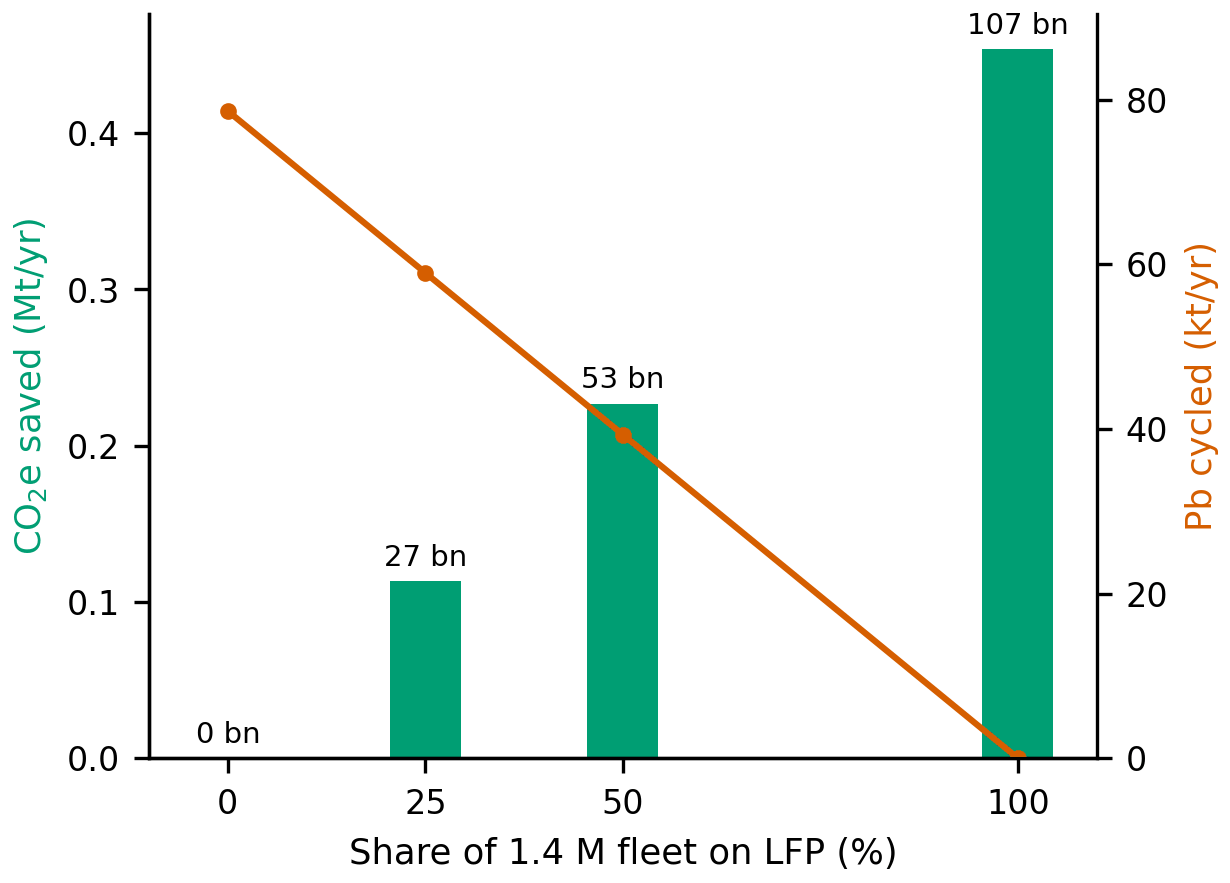
\includegraphics[width=0.5\textwidth]{fig6_policy.png}
\caption{Conversion scenarios: CO$_2$e saved (bars; labels give the operator support needed, $10^9$ BDT) and lead cycled through recycling (line) versus the share of the fleet on LFP.}
\label{fig:policy}
\end{figure}
